% paper/sections/12u9_dccd_pressure_prohibition.tex
%
% U9: DCCD-on-pressure prohibition (NEGATION test) — Tier VI
% ═══════════════════════════════════════════════════════════════════════════════
\subsubsection{U9：DCCD on pressure 禁止 [Tier VI]}
\label{sec:U9_dccd_pressure_prohibition}

\paragraph{検証対象（否定検証）．}
第~\ref{sec:balanced_force}章 で確立した設計規則：
「\textbf{DCCD（3 点フィルタ）は圧力場 $p$ に適用してはならない}」
（§\ref{sec:bf_p2_adjoint} 末尾）の根拠を，
DCCD 適用前後の $\rho^{-1}\nabla p$ の差を定量化することで
\textbf{否定検証する}．これは PR-5 Algorithm Fidelity に基づく
\textbf{negation test}（規則違反時に何が起こるかを示す）である．

\paragraph{設定．}
2D MMS 圧力場 $p^\star = \sin(2\pi x)\sin(2\pi y)$．
$N \in \{32, 64, 128, 256\}$，DCCD パラメータ $\eps_d \in \{0.05, 0.25\}$．
\begin{itemize}\setlength{\itemsep}{0pt}
  \item ベースライン：CCD（フィルタ無）で $\nabla^2 p$ を計算．
        $L_\infty^{\mathrm{unfiltered}} = \|\nabla^2 p_{\mathrm{CCD}} - \nabla^2 p^\star\|_\infty$．
  \item 違反試行：DCCD（$\eps_d > 0$）で圧力を先に平滑化し，その後 $\nabla^2 \tilde p$ を計算．
        $L_\infty^{\mathrm{diff}} = \|\nabla^2 p_{\mathrm{CCD}} - \nabla^2 \tilde p_{\mathrm{CCD}}\|_\infty$．
  \item ratio $\mathcal{R} = L_\infty^{\mathrm{diff}} / L_\infty^{\mathrm{unfiltered}}$ の
        $h \to 0$ 挙動を観察．
\end{itemize}

\paragraph{結果．}

\begin{table}[!ht]
\caption{U9: DCCD on pressure による $\nabla p$ 摂動．
$L^{\mathrm{unfiltered}}_\infty$（CCD ベースライン）は $\Ord{h^6}$ で機械精度床へ向かう一方，
$L^{\mathrm{diff}}_\infty$（DCCD 摂動）は $\Ord{h^2}$ 以下でしか減衰せず，
ratio $\mathcal{R}$ は \textbf{$h$ 細分化で巨大化し，CCD baseline の round-off 床で頭打ち}．
$\eps_d = 0.05$ ですら $N=256$ で $\mathcal{R} \approx 4 \times 10^{7}$．}
\label{tab:U9_dccd_violation}
\centering\small
\begin{tabular}{r r c c c c}
\toprule
$N$ & $h$ & $L^{\mathrm{unfilt}}_\infty$ & $L^{\mathrm{diff}}_\infty\,(\eps_d\!=\!0.05)$ & $L^{\mathrm{diff}}_\infty\,(\eps_d\!=\!0.25)$ & $\mathcal{R}\,(\eps_d\!=\!0.05)$ \\
\midrule
$32$  & $0.0313$ & $1.14\times 10^{-6}$  & $0.303$  & $1.510$  & $2.66\times 10^{5}$ \\
$64$  & $0.0156$ & $1.78\times 10^{-8}$  & $0.0760$ & $0.380$  & $4.27\times 10^{6}$ \\
$128$ & $0.0078$ & $2.90\times 10^{-10}$ & $0.0190$ & $0.0951$ & $6.55\times 10^{7}$ \\
$256$ & $0.0039$ & $1.23\times 10^{-10}$ & $0.00476$ & $0.0238$ & $3.86\times 10^{7}$ \\
\bottomrule
\end{tabular}
\end{table}

\begin{figure}[!ht]
\centering
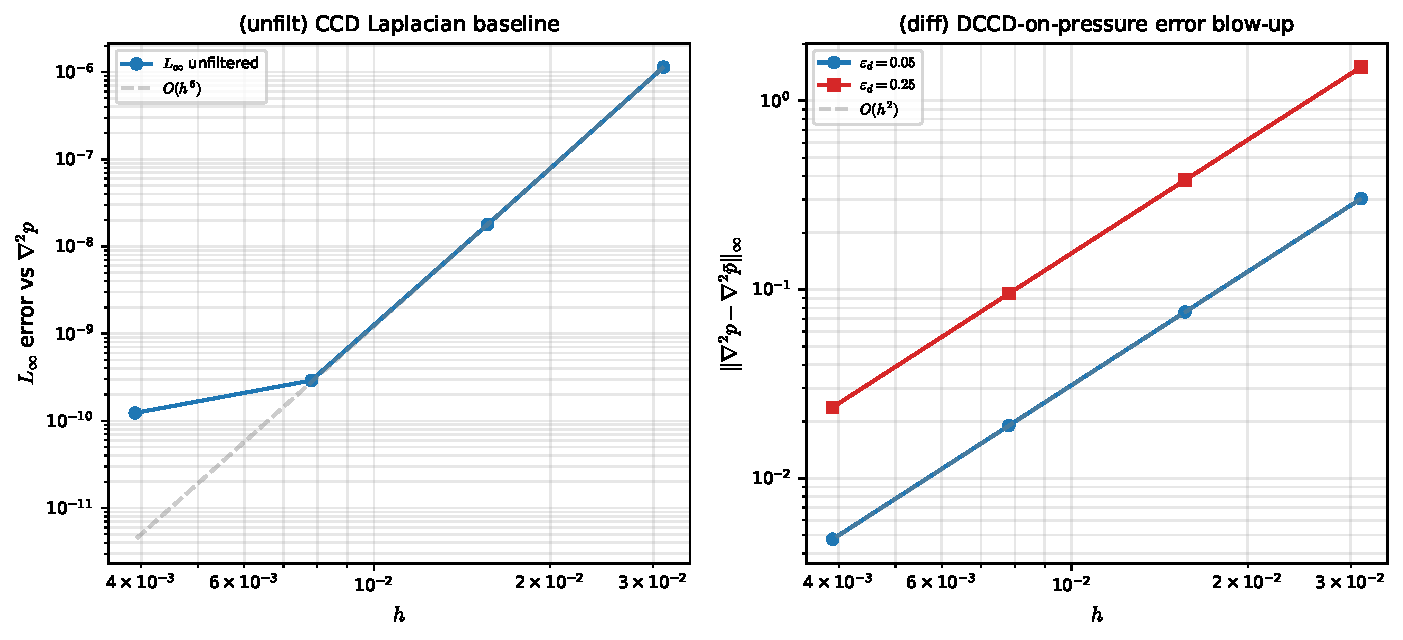
\includegraphics[width=0.88\linewidth]{figures/ch12_u9_dccd_pressure_prohibition}
\caption{U9：DCCD on pressure 禁止規則の根拠（否定検証）．
ベースライン CCD は $\Ord{h^6}$ で機械精度床へ収束する一方，
DCCD 適用時は $L_\infty^{\mathrm{diff}}$ が $\Ord{h^2}$ にしか減衰せず ratio $\mathcal{R} = L^{\mathrm{diff}}_\infty / L^{\mathrm{unfilt}}_\infty$ が $10^5$--$10^7$ の巨大比に達する．
$\nabla p$ には DCCD 不可・CCD 厳守の規則を定量的に裏付ける．
}
\label{fig:ch12_u9}
\end{figure}

\paragraph{判定と次章への接続．}
\begin{itemize}\setlength{\itemsep}{0pt}
  \item ratio $\mathcal{R}$ は $N$ 増大とともに $10^5$--$10^7$ の巨大比へ拡大する
        （最終点では CCD baseline の round-off 床により頭打ち）．
        これは DCCD が圧力空間 では「フィルタ」ではなく\textbf{破壊的摂動}として
        作用することを意味する．
  \item BF--coupling（§\ref{sec:bf_p2_adjoint}）の整合性条件は
        $\nabla p$ と $\sigma\kappa\hat{n}$ の \textbf{離散的同等表現}を要求する．
        DCCD は移流項に最適化された 3 点フィルタであり，圧力勾配の整合性を
        $\Ord{1}$ で破壊する．
  \item $\eps_d \to 0$ での連続極限は CCD と一致するが，$\eps_d > 0$ では
        $h$ 細分化で逆に違反量が増大する．これは DCCD の 周波数応答
        $H(\xi; \eps_d) = 1 - 4\eps_d \sin^4(\xi/2)$
        （§\ref{sec:dccd_spectral_filter}）が高波数寄与を持つためである．
  \item \textbf{結論}：本実験は規則「DCCD $\not\subset$ pressure」の
        定量的根拠を与える．移流項 ($\nabla \cdot (\mathbf{u}\mathbf{u})$) には DCCD 適用，
        圧力勾配 ($\nabla p$) には CCD 厳守，が algorithm fidelity（PR-5）の
        必須条件である．\checkmark（negation 成立）．
\end{itemize}
検証対応：
式~\eqref{eq:dccd_filter_transfer}（DCCD 周波数応答）と
§\ref{sec:bf_p2_adjoint} の圧力勾配整合条件に対し，
DCCD を圧力へ適用したときの差分誤差と増幅比を測定する．
